\chapter{Marco Teórico y herramientas de desarrollo}

Como mencionamos anteriormente, uno de los principales obstáculos para realizar predicciones a series de tiempo con niveles de agregación o jerarquía es garantizar su coherencia en todos los niveles. Esto es, que al agregar las predicciones, estas sean consistentes con la propia jerarquía. En este capítulo analizaremos algunas de las formas más utilizadas para conciliar predicciones de series de tiempo jerárquicas.

Utilizaremos la jerarquía de la figura \ref{fig:jerar_ex} y la siguiente notación tomada de \cite{abolghasemi2020model}:

\begin{itemize}
    \item $m$: total de nodos de la serie 
    \item $m_i$: total de nodos en el nivel i
    \item $k$: niveles de la jerarquía
    \item $n$: observaciones en una serie
    \item $y_t$: t-ésima observación 
    \item $\hat{y_t}$: predicción de la t-ésima observación
    %\item $Y_{x,t}$: serie del nodo x en el tiempo t
    %\item $\hat{Y}_{x,n}(h)$: vector de predicciones con h saltos por delante para la serie $Y_x$ con n observaciones
    \item $\textbf{Y}_{i,t}$: vector de todas las obervaciones del nivel i
    \item $\hat{\textbf{Y}}_{i,t}(h)$: vector de predicciones con h saltos por delante para el nivel i
    %\item $\textbf{Y}_t$: vector columna con todas las observaciones
    %\item $\hat{\textbf{Y}}_n(h)$: predicción con h saltos por delante de toda la serie basada en n observaciones
    \item $\Tilde{Y}_n(h)$: vector de predicciones conciliadas con h saltos por delante para el nivel i
\end{itemize}

\begin{figure}
    \centering
    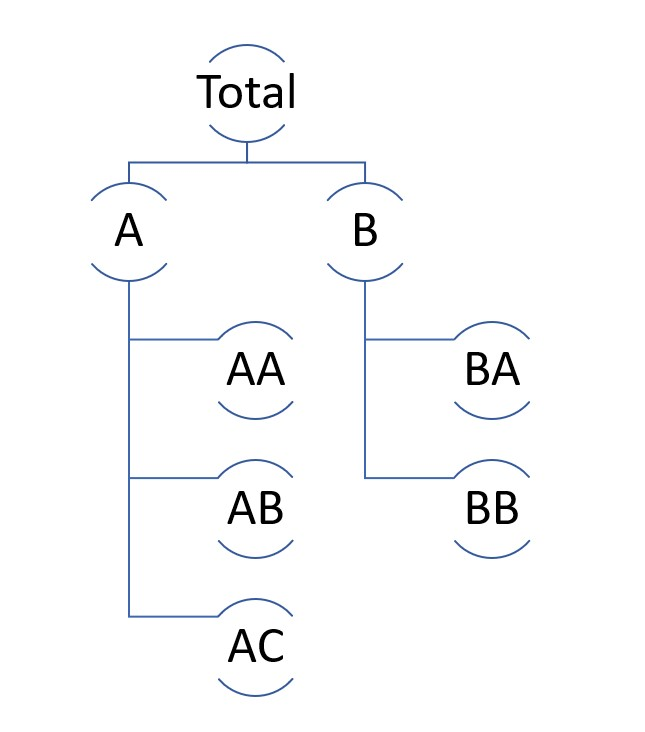
\includegraphics[width=0.5\textwidth]{imgs/jerar_ex.jpg}
    \caption{Jerarquía ejemplo}
    \label{fig:jerar_ex}
\end{figure}

\section{Técnicas de conciliación en una jerarquía}

Tradicionalmente, las predicciones en series de tiempo de jerarquía requieren de seleccionar un nivel en la estructura para realizar la predicción y de ahí agregarla (niveles superiores) o desagregarla (niveles inferiores) para los otros niveles. 

\subsection{Buttom-up}

El método de ''abajo-arriba'' es uno de los más simples pues únicamente implica realizar la predicción en la base de la jerarquía. Una vez hecho esto, las predicciones se suman para conformar la información de los niveles superiores.

La principal ventaja de esta técnica es que considera el nivel más bajo de la serie por lo que no perdemos información atómica. No obstante, esta técnica tiene la desventaja de ser muy ruidosa.

Por ejemplo, con la jerarquía de la figura \ref{fig:jerar_ex} calcularíamos primero las predicciones (con h saltos por delante) de la base: $\hat{Y}_{AA,h}$, $\hat{Y}_{AB,h}$, $\hat{Y}_{AC,h}$, $\hat{Y}_{BA,h}$ y $\hat{Y}_{BB,h}$. Luego las sumaríamos para obtener la predicción conciliada del total de diferentes maneras como:

\begin{equation}
    \Tilde{Y}_h = \hat{Y}_{AA,h} + \hat{Y}_{AB,h} + \hat{Y}_{AC,h} + \hat{Y}_{BA,h} + \hat{Y}_{BB,h}
\end{equation}

\begin{equation}
    \Tilde{Y}_h = \Tilde{Y}_{A,h} + \Tilde{Y}_{B,h}
\end{equation}

Donde las predicciones conciliadas para los niveles A y B se calculan al sumar las predicciones base de sus elementos. 


\subsection{Top-down}

Por su parte, el método de ''arriba-abajo'' genera una única predicción en el nivel más agregado la cual se desagrega a los niveles inferiores. Para realizar lo anterior, se utilizan proporciones que ayudan a determinar cómo manejar la predicción en los distintos niveles.

La principal ventaja de este método es su simplicidad al usar una sola predicción, la del total. Sin embargo, su defecto es la pérdida de información de los niveles inferiores como patrones de temporada o eventos especiales por mencionar algunos.

En este caso, para la jerarquía de la figura \ref{fig:jerar_ex}, primero calculamos la predicción en la cima, luego calculamos las predicciones en la base usando las proporciones $p_1, p_2, p_3, p_4$ y $p_5$ de la siguiente manera: $\Tilde{Y}_{AA,t} = p_1\hat{Y}_t$, $\Tilde{Y}_{AB,t} = p_2\hat{Y}_t$, $\Tilde{Y}_{AC,t} = p_3\hat{Y}_t$, $\Tilde{Y}_{BA,t} = p_4\hat{Y}_t$, $\Tilde{Y}_{BB,t} = p_5\hat{Y}_t$. 

Para calcular las proporciones existen 2 métodos populares: promedio de las proporciones históricas y proporciones de los promedios históricos. El primero tiene la fórmula indicada en la ecación \ref{ec:avg_p}, mientras que el segundo se expresa como la ecuación \ref{ec:p_avg}. Donde j va de 1 a $m_k$.

\begin{equation}
    p_j = \frac{1}{n} \sum_{t=1}^{n} \frac{Y_{j,t}}{Y_t}
    \label{ec:avg_p}
\end{equation}

\begin{equation}
    p_j = \frac
            {\sum_{t=1}^{n}Y_{j,t}}
            {\sum_{t=1}^{n}Y_t}
    \label{ec:p_avg}
\end{equation}

\subsection{Middle-out}

Esta técnica junta las dos anteriores a partir de un nivel pivote. Los niveles superiores se calculan con la técnica ''abajo-arriba'' mientras que los niveles inferiores con la técnica ''arriba-abajo
''. Su principal desventaja es que el analista debe elegir el nivel pivote y sustentar su elección.

Como podemos observar, el camino sugerido para la conciliación de pronósticos es primero realizar la predicción ($\hat{Y_t}$) y luego conciliar por alguno de los métodos anteriores ($\Tilde{Y_t}$)

Sin embargo, la 3 técnicas descritas tienen el detalle de que se enfocan en un nivel particular de agregación para hacer el pronóstico. Esto tiene la consecuencia de ignorar información relevante de los otros niveles. Por ello, las tecnicas que combinan las bondades de las 3 anteriores y consideran la información en todos los niveles de la jerarquía son superiores. Estas técnicas son llamadas de combinación óptima, pues mediante pesos calculados, combinan las predicciones obtenidas garantizando la coherencia requerida. Estos pesos dependen solo de la jerarquía y no de los datos.

Es importante destacar que se facilita la visualización de la agregación de series de tiempo jerárquicas con el uso de notación matricial. 

La figura \ref{fig:jerar_ex} en el tiempo t se puede representar de la siguiente manera:

\begin{equation}
    \begin{bmatrix}
    Y_t\\
    Y_{A,t}\\
    Y_{B,t}\\
    Y_{AA,t}\\
    Y_{AB,t}\\
    Y_{AC,t}\\
    Y_{BA,t}\\
    Y_{BB,t}\\
    \end{bmatrix} = 
    \begin{bmatrix}
    1,1,1,1,1\\
    1,1,1,0,0\\
    0,0,0,1,1\\
    1,0,0,0,0\\
    0,1,0,0,0\\
    0,0,1,0,0\\
    0,0,0,1,0\\
    0,0,0,0,1\\
    \end{bmatrix}
    \begin{bmatrix}
    Y_{AA,t}\\
    Y_{AB,t}\\
    Y_{AC,t}\\
    Y_{BA,t}\\
    Y_{BB,t}\\
    \end{bmatrix}
\end{equation}

De manera compacta, la serie \textbf{$Y_t = SY_{k,t}$} se calcula con la matriz S de agregación de $m$ x $m_k$ y el vector $Y_{k,t}$ con las observaciones en el nivel k de la jerarquía en el tiempo t. En este caso, las del último nivel. Notemos que estas últimas se expresan con la matriz identidad.

\section{ML Framework}

El framework para realizar pronósticos de series de tiempo con ML es similar al visto en el curso. Destacamos el camino sugerido por \cite{hyndman2018forecasting} el cual comienza con la preparación de los datos, su visualización y su descripción con un modelo; posteriormente el modelo se entrena con los datos de entrenamiento; finalmente, se evalúa su desempeño con una muestra separada de prueba. Si el desempeño no es satisfactorio, realizamos modificaciones en los primeros pasos. Con un modelo apropiado, entonces se realizan las predicciones.

\subsection{Evaluación de residuales}

Cuando hacemos predicciones de series de tiempo, comúnmente usamos toda la información previa al punto de predicción. Es decir, un pronóstico $\hat{y_t}$ involucra toda la serie hasta t-1. Aunque existen diversas formas de construir la predicción, se utiliza el acercamiento naive como punto de comparación. Este acercamiento propone como predicción $\hat{y_t}=y_{t-1}$. A los pronósticos les llamamos valores ajustados, pues involucran esa información previa.

Con los valores ajustados de una serie, podemos checar el ajuste al compararlo contra el valor real en el mismo tiempo t. La diferencia entre estos valores se llama residual y nos permite determinar si el modelo está capturando información relevante de los datos.

Un buen modelo de predicción de series de tiempo tiene las siguientes características en sus residuales: no están correlacionados y tienen media 0. Cuando esto no sucede, entonces el modelo puede ser mejorado. Adicionalmente, resulta beneficioso que los residuales tengan varianza constante y que su distribución sea normal, pues facilitan el cálculo de intervalos de predicción \cite{hyndman2018forecasting}.

\subsection{Separación de datos}


    \begin{figure}[t]
    \centering

      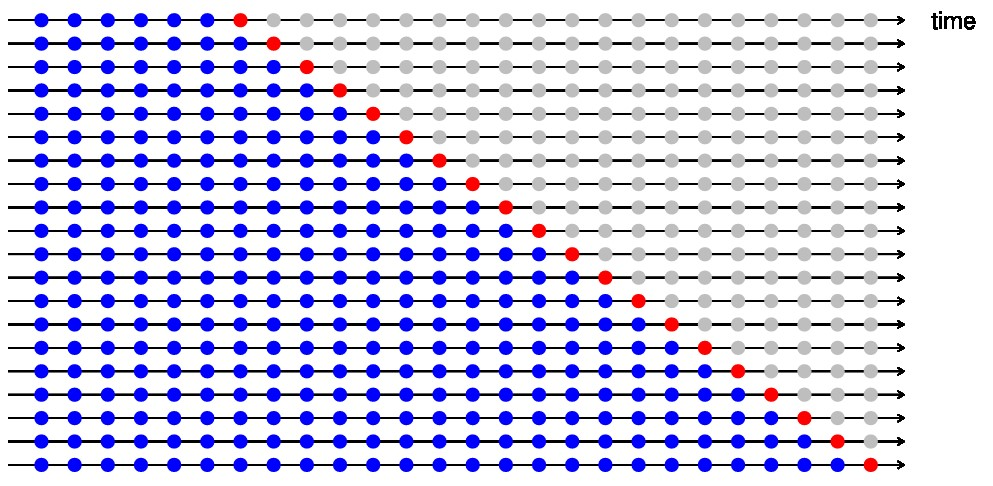
\includegraphics[width=55mm]{imgs/train_cv1.jpg}
      \caption{Validación cruzada a 1 tiempo en el futuro. Los cortes de entrenamiento comprenden las observaciones azules. Los cortes de prueba se construyen con la observación roja.}
      \label{fig:train_cv1}

      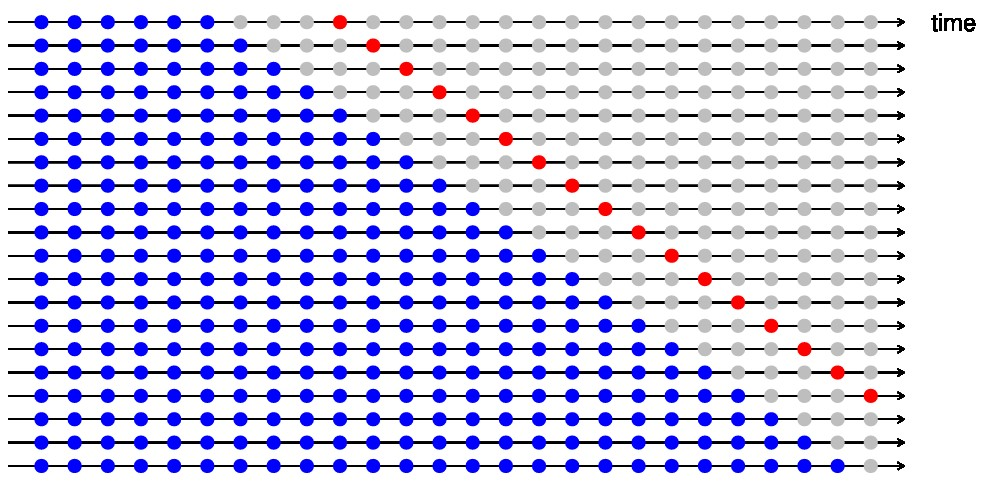
\includegraphics[width=55mm]{imgs/train_cv2.jpg}
      \caption{Validación cruzada a h tiempos en el futuro. Los cortes de entrenamiento comprenden las observaciones azules. Los cortes de prueba se construyen con la observación roja.}
       \label{fig:train_cv2}

    \end{figure}
    
Para evaluar las predicciones de un modelo bien ajustado necesitamos valores reales, pues la información de los residuales subestima el peso de un error predictivo. Por ello, utilizamos una muestra de entrenamiento para ajustar el modelo y una muestra separada para probar su capacidad predictora. 

Comunmente, la separación en series de tiempo utiliza la siguiente forma: la muestra de entrenamiento comprende las observaciones $\{y_1,...,y_t\}$, mientras que la muestra de prueba va de $\{y_{t+1}, ...\}$ en adelante. De esta manera, podemos hablar del error de predicción de un pronóstico como la diferencia entre el valor observado y el propio pronóstico $e_t = y_t - \hat{y_t}$. 

Dicho lo anterior, la manera de implementar validación cruzada en series de tiempo implica garantizar que los cortes de entrenamiento y prueba tengan la estructura previamente descrita: la muestra entrenamiento siempre tiene información previa a la muestra de prueba. Normalmente construimos la muestra de prueba con una sola observación en el tiempo t mientras que la muestra de entrenamiento tiene las observaciones hasta t-1. Esto se puede ver en la figuras \ref{fig:train_cv1}. Por su parte la figura \ref{fig:train_cv2} indica la misma idea cuando el pronóstico es h tiempos adelante.


Destacamos la diferencia entre residuales y errores de predicción ya que los primeros solo se calculan en la muestra de entrenamiento con diferencia de 1 tiempo t, pero los segundos se calculan en la muestra de prueba con diferencia de h tiempos, pues reflejan el pronóstico en el futuro deseado.

Finalmente, utilizamos algunas medidas tradicionales de ML para medir el desempeño de las predicciones, en particular, cuando las observaciones están en la misma escala podemos usar MAE o RMSE. Cabe destacar que es común la ausencia de misma escala en los datos por lo que ajustes como MASE o RMSSE, donde se toma en cuenta qué tan alejada fue la predicción respecto al modelo naive, son preferibles \cite{hyndman2018forecasting}.


\section{Base de datos}

Para ejemplificar la conciliación de series de tiempo jerárquica, se usará la base de datos (\textbf{tourism}), que  contiene los viajes nocturnos trimestrales desde el primer trimestre de 1998 hasta el cuarto trimestre de 2016 en Australia. Las variables de esta base de datos son:

\begin{itemize}
    \item \textbf{Quarter:} Trimestre
    \item \textbf{State:} 8 Estados y territorios de Australia.
    \item \textbf{Region:} 76 Regiones formadas a partir de la agregación de Áreas Locales Estadísticas (SLA), definnidas por autoridades de turismo estatales.
    \item \textbf{Purpose:} 4 Propósitos de visita ("Holiday", "Visiting friends and relatives", "Business", "Other reason").
    \item \textbf{Trips:} Viajes nocturnos en miles.
\end{itemize}

En \textit{tourism} se tiene una jerarquía dentro de sus variables, para cada Estado, se pueden tener distintas Regiones contenidas. En R, la base de datos es parte del paquete \textit{tsibble} que se explicará más adelante. Como un breve EDA, tenemos que la base contiene 24,320 registros.  Al ver todas las series de tiempo que se pueden generar hay que considerar los distintos niveles de agregación:

\newpage

Al considerar las estados podemos contar 8 series de tiempo a un nivel estado:

    \begin{figure}[!h]
    \centering
      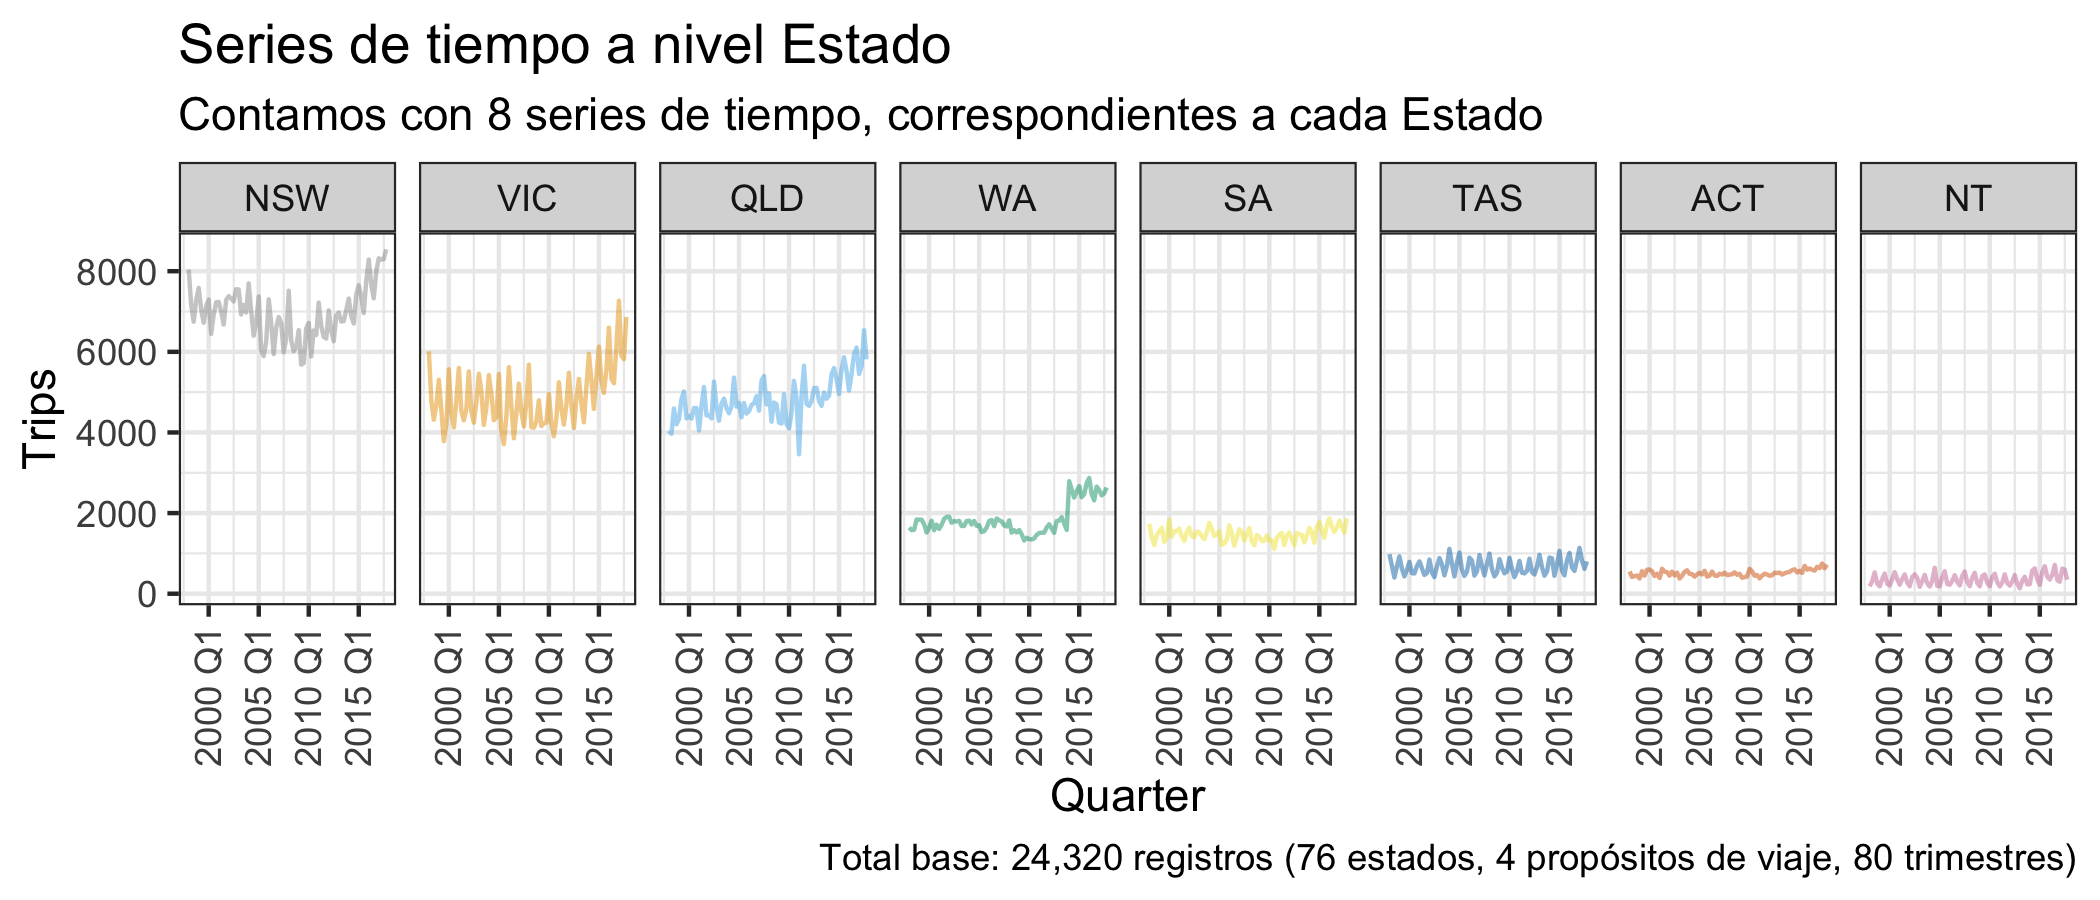
\includegraphics[width=120mm]{imgs/01_ts_state.png}
      \label{fig:snowyplot}
    \end{figure}
    
Si añadimos un nivel extra a la serie de tiempo, es decir consideramos todas las posibles series de tiempo a nivel estado y propósitos podemos tener 32 series de tiempo:

    \begin{figure}[!h]
    \centering
      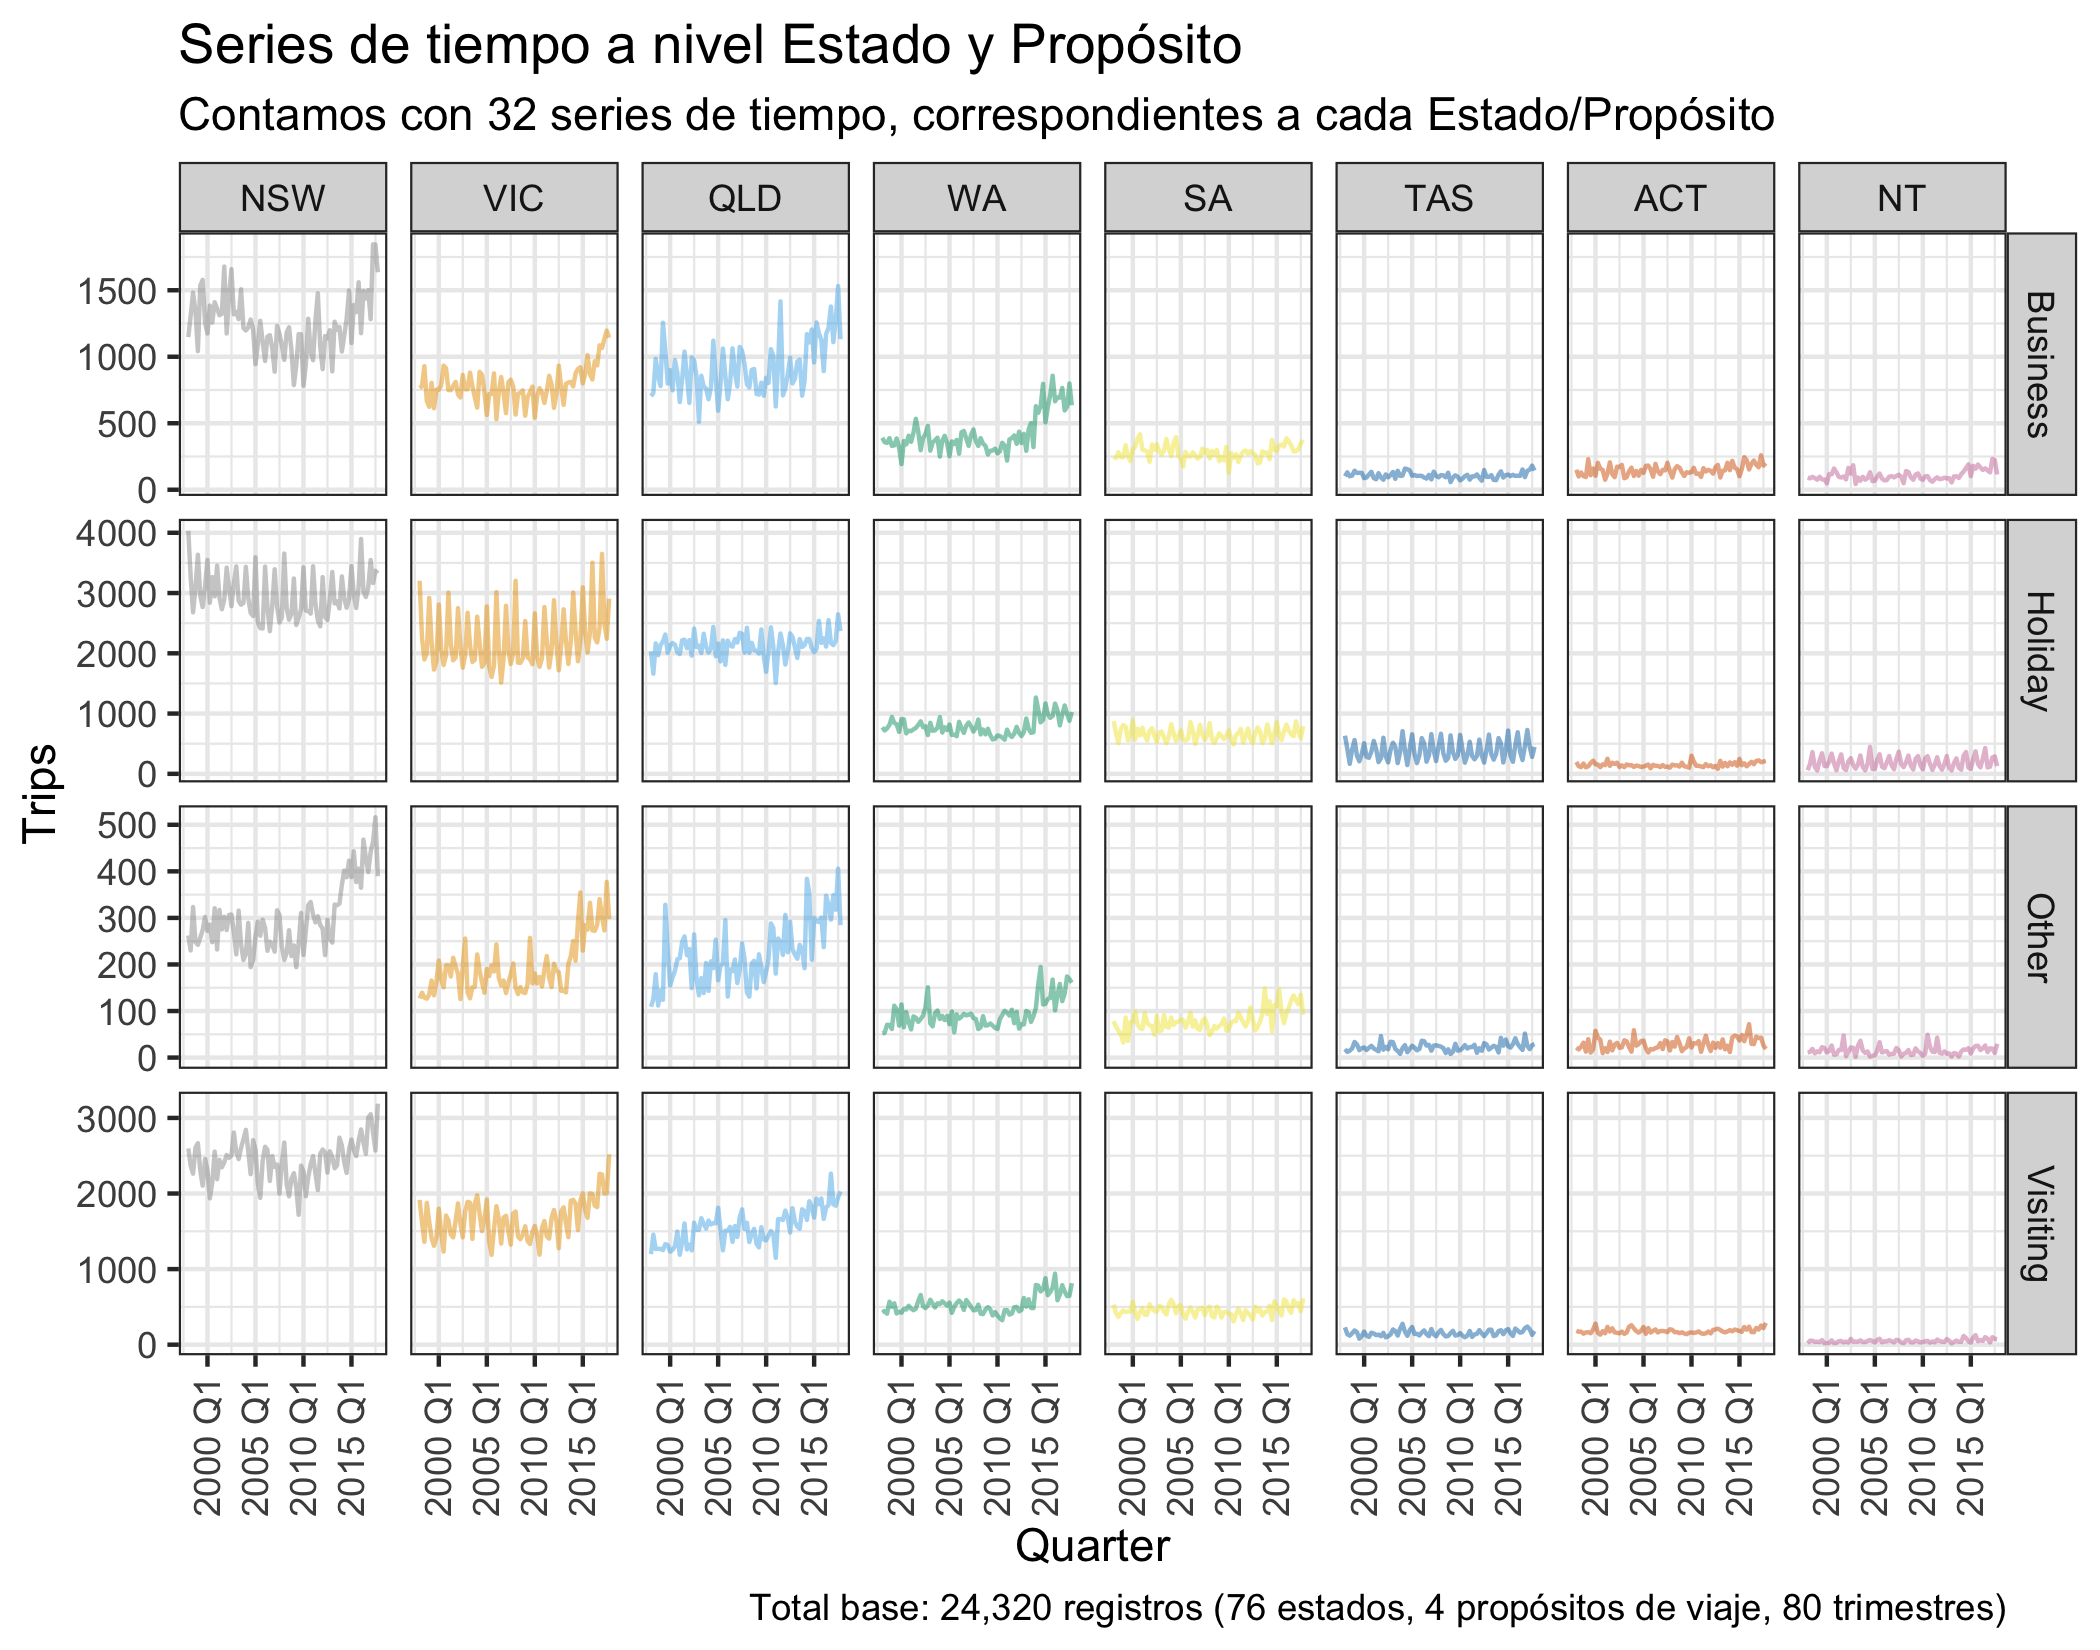
\includegraphics[width=120mm]{imgs/02_ts_state_purpose.png}
      \label{fig:snowyplot}
    \end{figure}
    
\newpage 

Finalmente, cuando consideramos el nivel de agregación más pequeño podemos llegar a un nivel región -  propósito donde podemos tener 304 series de tiempo:

    \begin{figure}[!h]
    \centering
      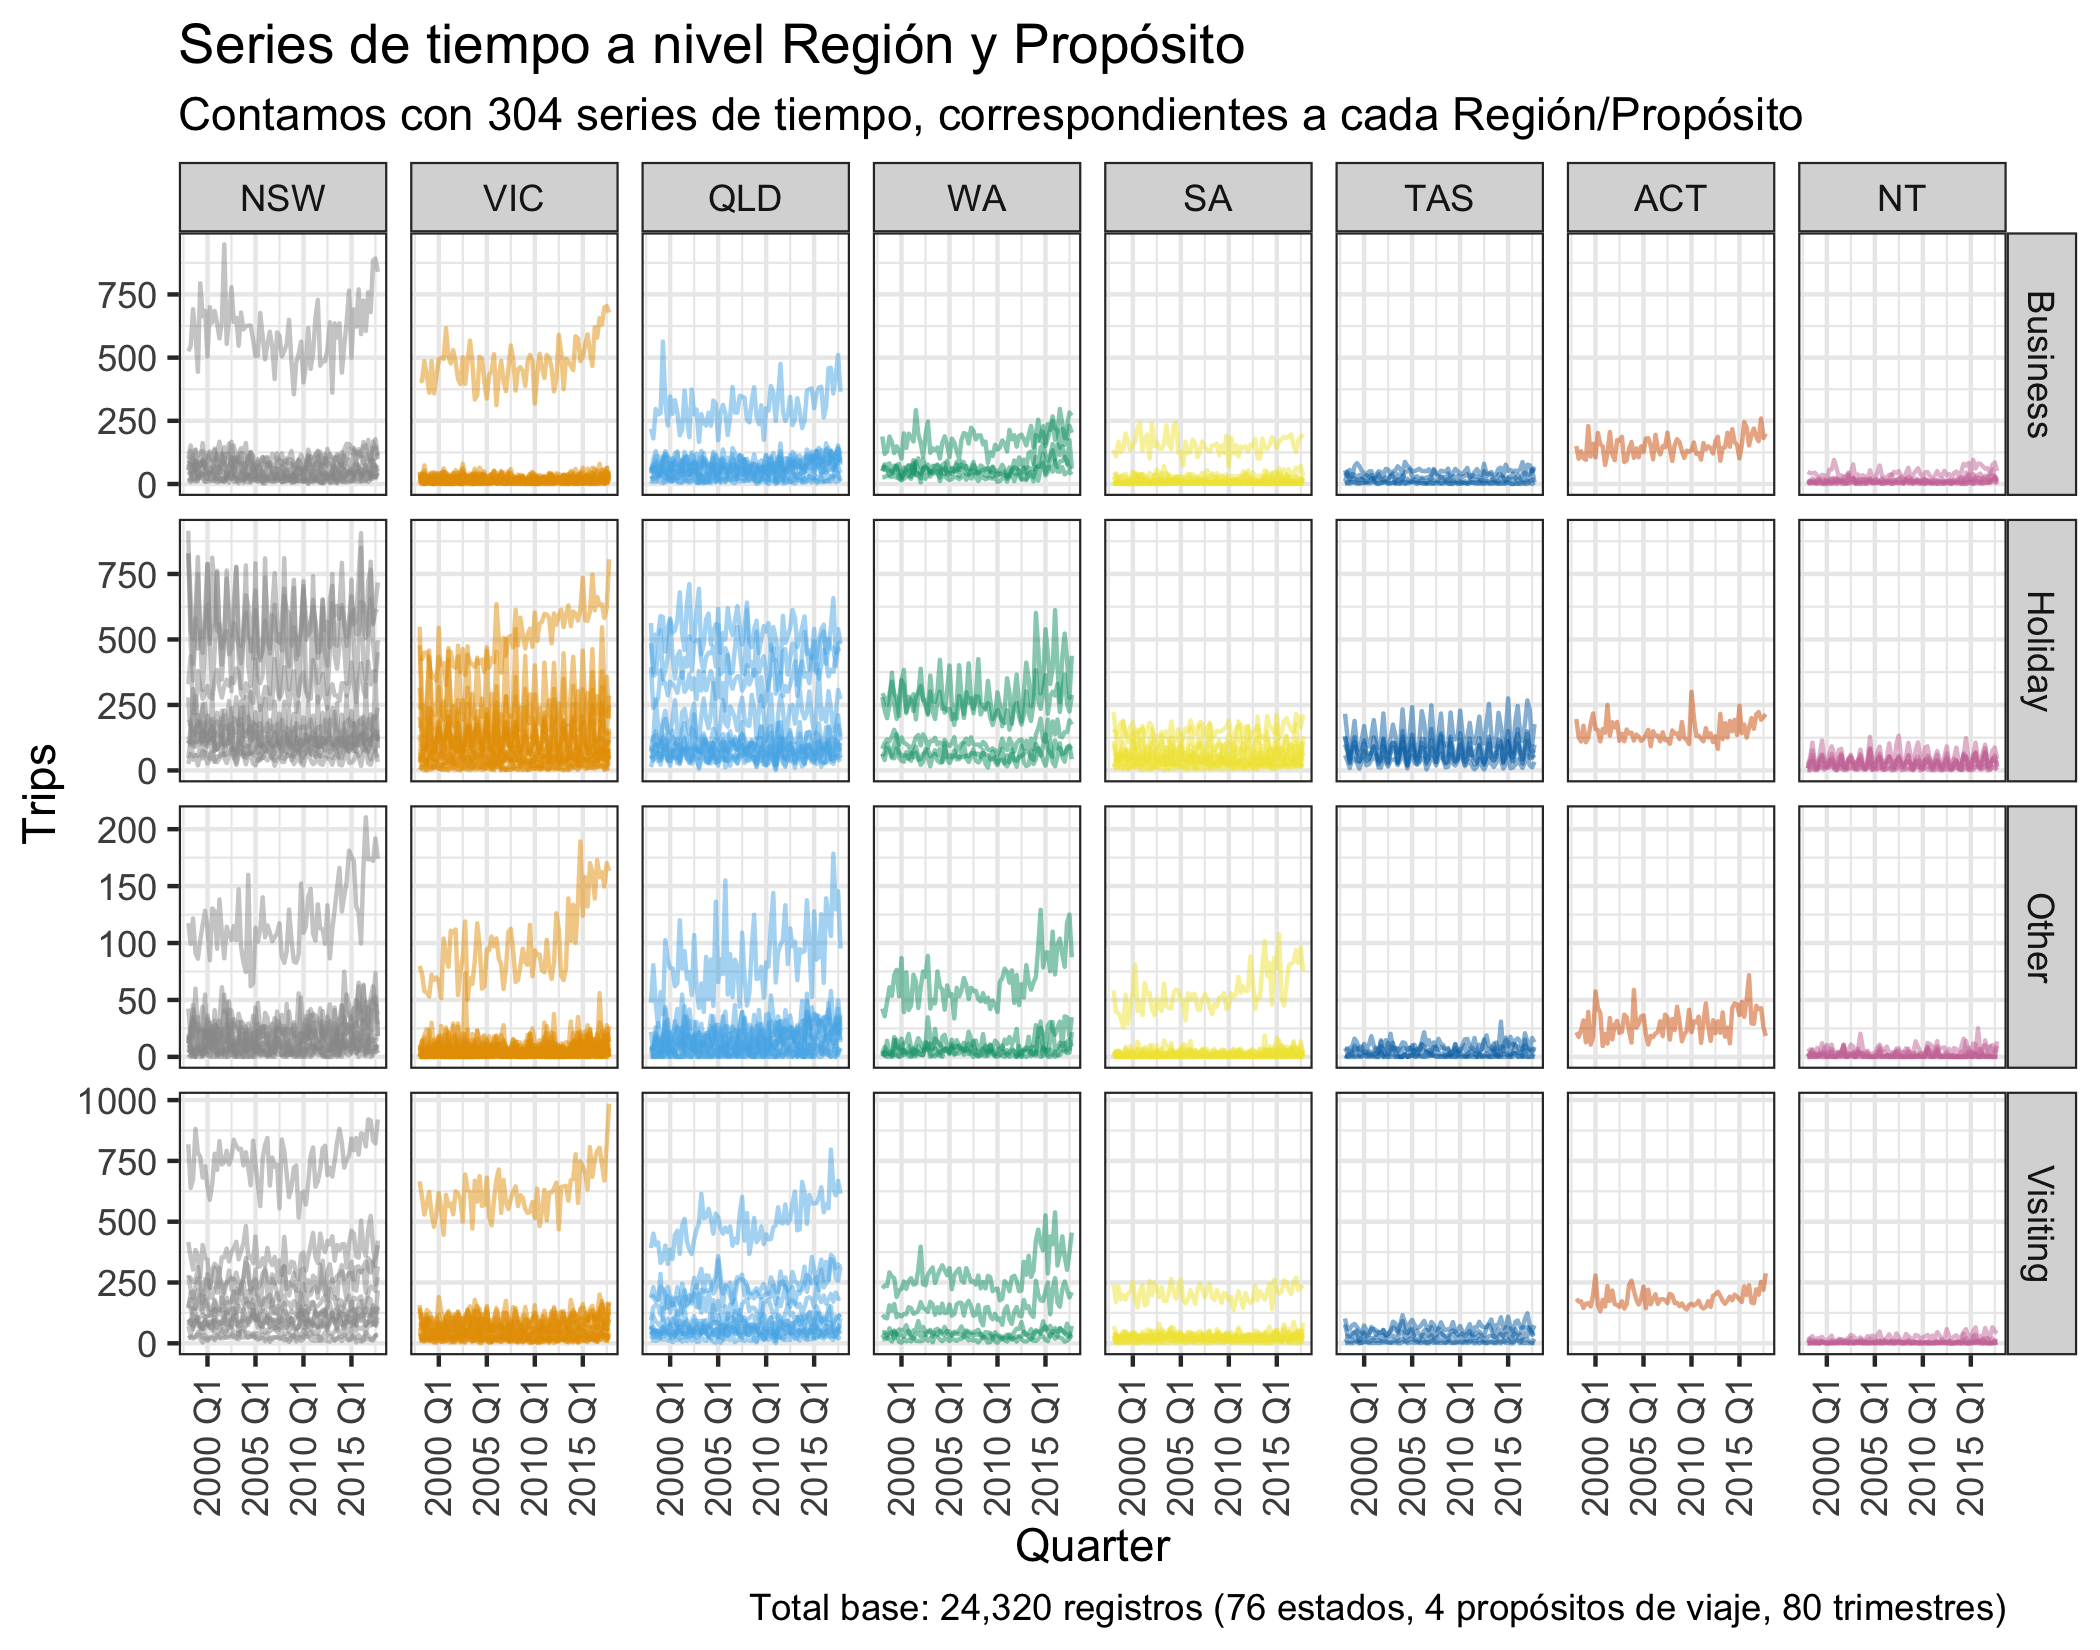
\includegraphics[width=120mm]{imgs/03_ts_region_purpose.png}
      \label{fig:snowyplot}
    \end{figure}

\newpage
    
\section{Paquetería empleada de R:}

Para resolver el problema tomamos la colección de paquetes de \textit{Tidyverts}, que es un simil de \textit{Tidyverse} y \textit{Tidymodels} enfocado en series de tiempo. Esta colección de paquetes tiene contribuciones de Rob Hyndman autor del libro \textit{Forecasting: Principles and Practice} \cite{hyndman2018forecasting}, donde se plantean temas de series de tiempo desde un punto de vista aplicado y enfocado a R. 

Los paquetes de \textit{tidyverts} permiten predicciones de series de tiempo con grupos. Por ejemplo \textit{tourism} tiene establecida por default la llave: \{Estado, Region, Propósito\} el cual nos lleva a contar los 304 grupos indicados anteriormente. La base de datos de \textit{tourism} empleada en este trabajo consiste en un objeto de tipo \textit{tsibble}, donde: 

\begin{itemize}
    \item \textbf{Indice (index):} es una variable con un orden inherente del pasado al presente (En la base corresponde a la variable Quarter). Las posibles opciones que se pueden utilizar son:
    \begin{itemize}
    \item Anual
    \item Trimestral
    \item Mensual
    \item Semanal
    \item Diario
    \item Subdiario (A varios niveles como hora y minuto)
\end{itemize}
    \item \textbf{Clave (key):} es un conjunto de variables que definen las unidades de observación a lo largo del tiempo. (En la base corresponde a las variables \{Estado, Region, Propósito\})
    \item \textbf{Mediciones:} corresponden a los valores (o unidades de medida) que vamos a pronosticar.
\end{itemize}

La colección contiene los siguientes paquetes:

\begin{minipage}{0.1\textwidth}
\hspace{\fill} 
\end{minipage}
\begin{minipage}{0.3\textwidth}

\includegraphics[height=2cm]{imgs/tsibble.png}
\end{minipage}
\begin{minipage}{0.5\textwidth}
\textbf{tsibble:}  Provee una clase \textit{tbl\_ts} para datos temporales. Adicional contiene funciones que permiten analizar estos objetos
\end{minipage}

\begin{minipage}{0.1\textwidth}
\hspace{\fill} 
\end{minipage}
\begin{minipage}{0.3\textwidth}

\includegraphics[height=2cm]{imgs/fable.png}
\end{minipage}
\begin{minipage}{0.5\textwidth}
\textbf{fable:}  Contiene una colección de modelos para realizar time series forecasting. Lo interesante es que fucionan con el framework de \textit{fable} proveido por el paquete \textit{fabletools}
\end{minipage}

\begin{minipage}{0.1\textwidth}
\hspace{\fill} 
\end{minipage}
\begin{minipage}{0.3\textwidth}

\includegraphics[height=2cm]{imgs/fable.png}
\end{minipage}
\begin{minipage}{0.5\textwidth}
\textbf{fable.prophet:}  Contiene wrapers para el paquete de prophet que permite que sean utilizados en el mismo flujo del framework
\end{minipage}

\begin{minipage}{0.1\textwidth}
\hspace{\fill} 
\end{minipage}
\begin{minipage}{0.3\textwidth}

\includegraphics[height=2cm]{imgs/feasts.png}
\end{minipage}
\begin{minipage}{0.5\textwidth}
\textbf{feasts:}  Provee una colección de características, métricas estadísticas y funciones para graficar que es compatible con el mismo framework
\end{minipage}


\begin{minipage}{0.1\textwidth}
\hspace{\fill} 
\end{minipage}
\begin{minipage}{0.3\textwidth}

\includegraphics[height=2cm]{imgs/fable.png}
\end{minipage}
\begin{minipage}{0.5\textwidth}
\textbf{fable.tools:}  Contiene las funcionalidades y herramientas core del \textit{fable} framework.
\end{minipage}

\section{Ejemplo del Framework tidyverts }

Con fines exploratorios se exhiben las principales funciones de tidyverts para series de tiempo. Principalmente, tenemos la funcion \textit{Model} que permite construir distintos modelos como se muestra en el siguiente código. En este caso, generamos 3 modelos distintos y comunes en la literatura de series de  tiempo (ARIMA, ETS, SNAIVE) para los 304 grupos:

\begin{lstlisting}
fit <- 
  tourism %>%
  filter(year(Quarter) <= 2014) %>% 
  model(
    snaive = SNAIVE(Trips ~ lag("year")),
    ets = ETS(Trips),
    arima = ARIMA(Trips)
  )
\end{lstlisting}

\begin{figure}[!h]
        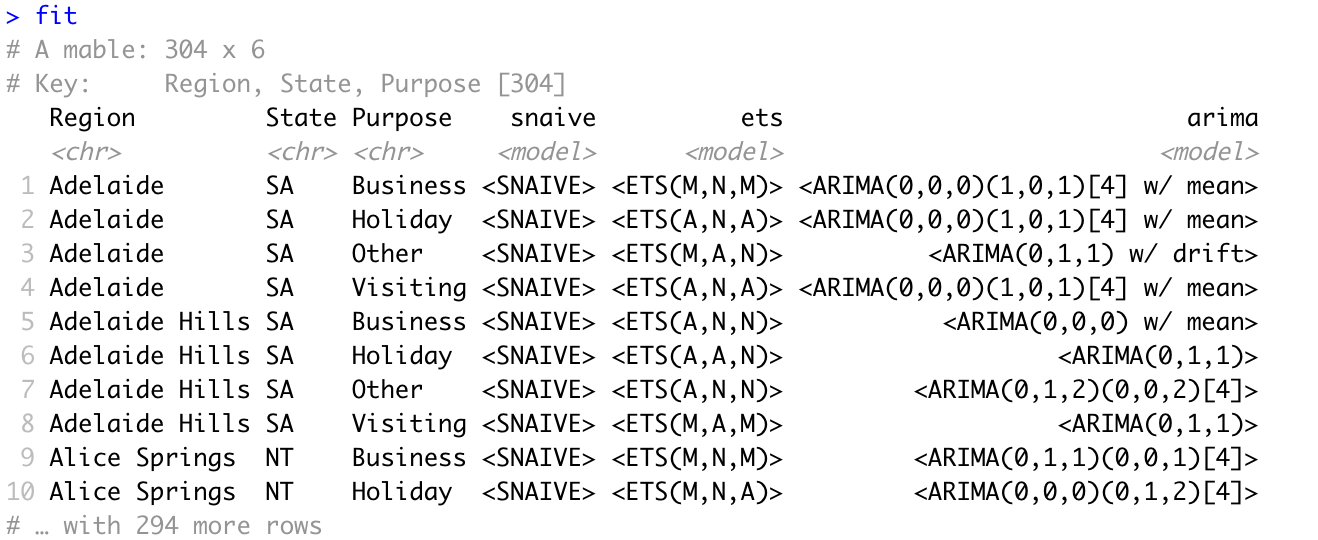
\includegraphics[width=120mm]{imgs/04_fit.png}
\end{figure}

Es importante notar en la línea 3 se aplica un filtro a los datos. Esto es reelevante por que es requerido para poder realizar predicciones y comparar con el dato verdadero

\newpage

Una ventaja de tidyverts, es que se puede analizar la especificacion para cada modelo en particular. Por ejemplo: Se puede seleccionar el modelo ARIMA para el grupo de \textbf{Region = Snowy Mountains} y \textbf{Purpose = Holiday}. Con esto vemos la especificacion del modelo, asi como sus respectivos  coeficientes con sus errores estándar. Adicionalmente, proporciona la log likelihood, AIC y BIC.

\begin{lstlisting}
fit %>%
  filter(Region == "Snowy Mountains", Purpose == "Holiday") %>%
  select(arima) %>%
  report()
\end{lstlisting}

\begin{figure}[!h]
        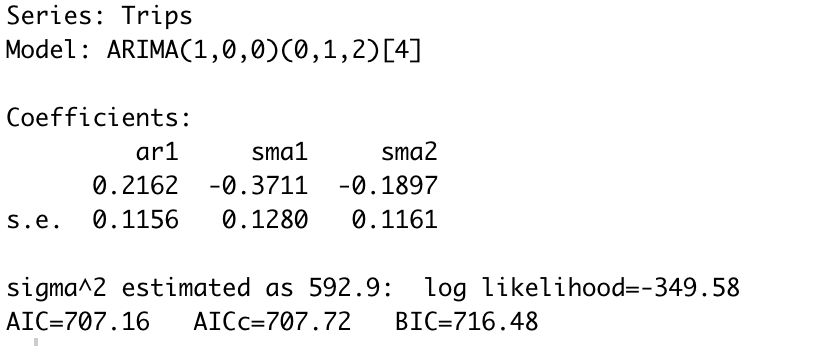
\includegraphics[width=75mm]{imgs/05_fit_arima.png}
\end{figure}

Además, podemos incluir predicciones (forecast) de la serie de tiempo para un periodo especificado:

\begin{lstlisting}
fit %>%
  filter(Region == "Snowy Mountains", Purpose == "Holiday") %>%
  forecast(h = "3 years")
\end{lstlisting}

\begin{figure}[!h]
        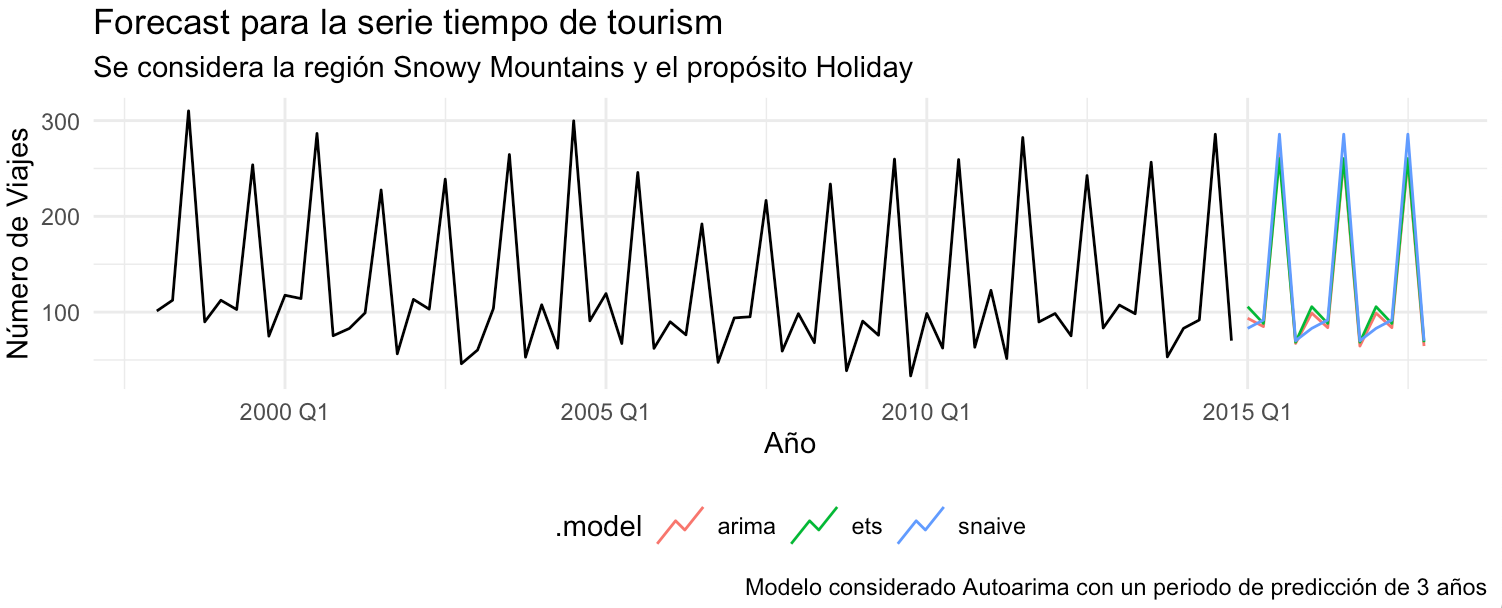
\includegraphics[width=120mm]{imgs/08_arima_plot.png}
\end{figure}

Adicionalmente, se puede determinar el error de esta predicción con la función \textit{accuracy}:

\begin{lstlisting}
accuracy(model\_for, tourism)
\end{lstlisting}

\begin{figure}[!h]
        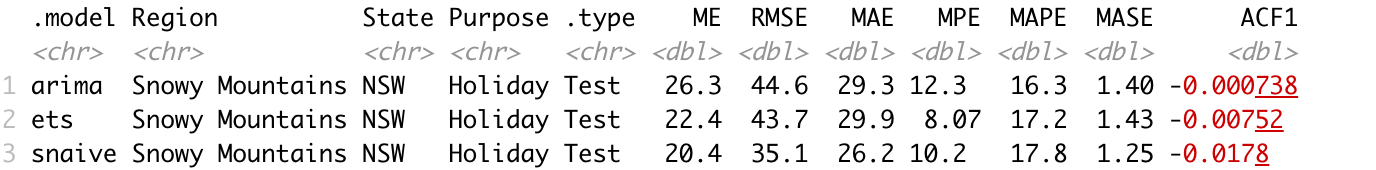
\includegraphics[width=120mm]{imgs/09_arima_error.png}
\end{figure}

\newpage

Algo interesante de este approach, es que se pueden utilizar funciones genéricas como \textit{glance}, \textit{coef} y \textit{augment}. La primera nos permite tener un "vistazo" de nuestro modelo ajustado. En este caso podemos para cada Región, Estado y Propósito los modelos especificados, su AIC, BIC, MAE, MASE, etc.

\begin{lstlisting}
fit %>%
  glance() %>% 
  arrange(MSE)
\end{lstlisting}

\begin{figure}[!h]
        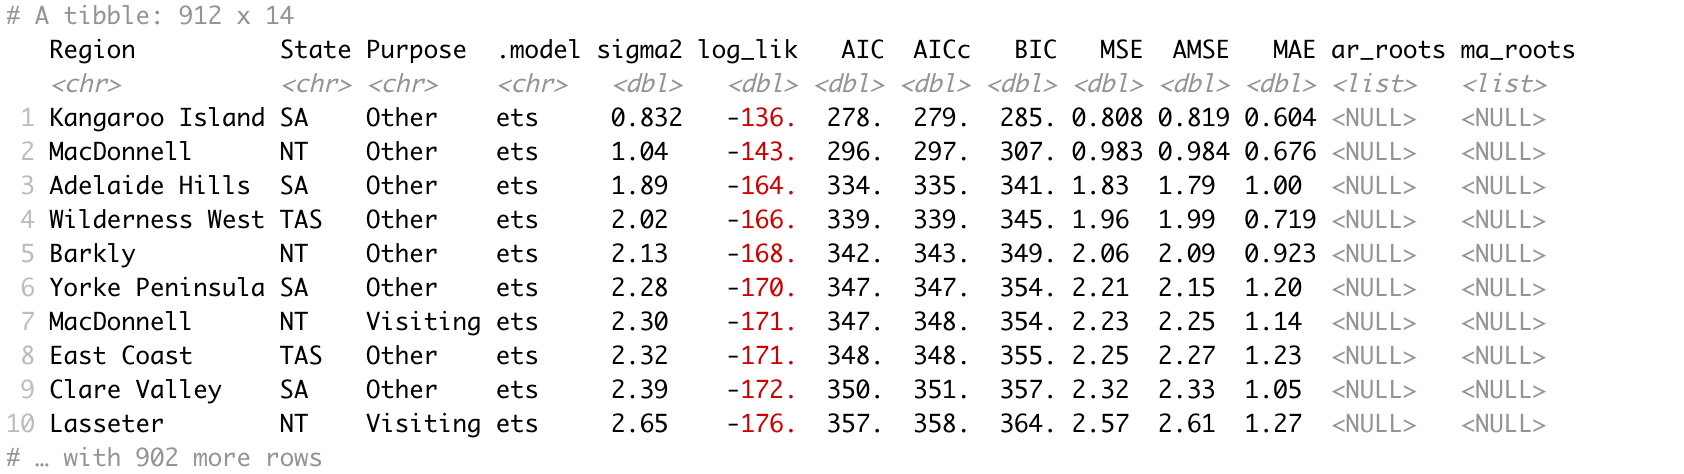
\includegraphics[width=110mm]{imgs/10_glance.png}
\end{figure}

Adicionalmente, es posible obtener el valor de los coeficientes que se estiman, así como su error estándard y su respectivo p-value.

\begin{lstlisting}
fit %>%
  select(Region, State, Purpose, arima) %>%
  coef()
\end{lstlisting}

\begin{figure}[!h]
        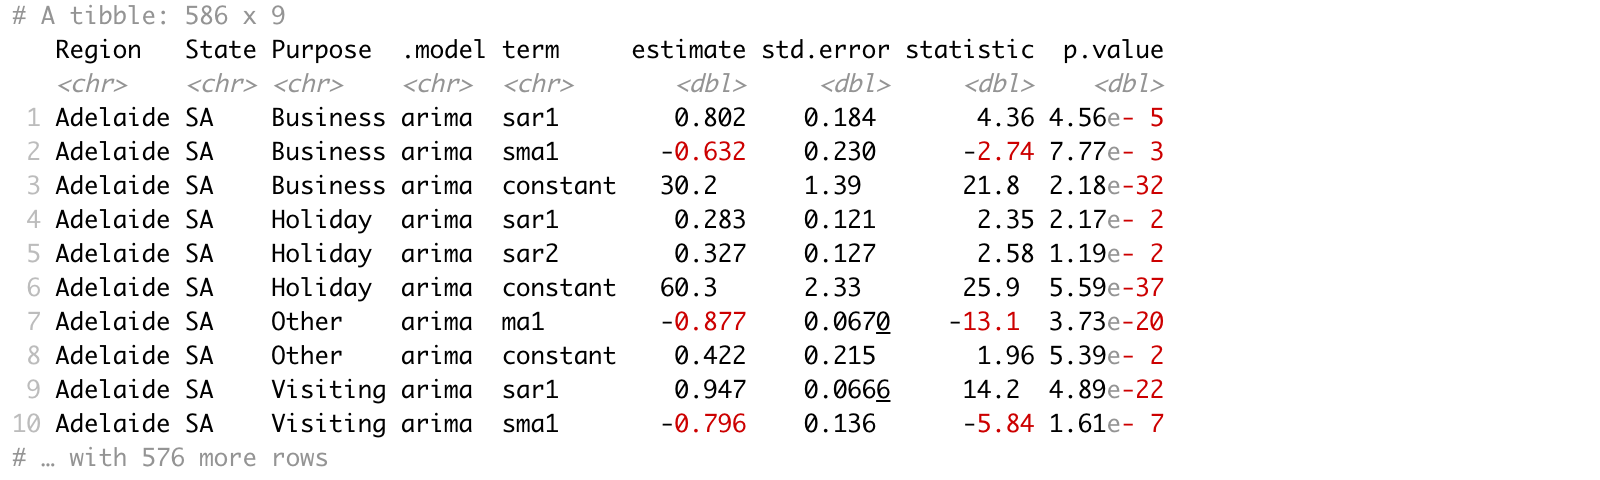
\includegraphics[width=110mm]{imgs/11_coef.png}
\end{figure}

Por último se puede observar el valor ajustado y el residual por observación y modelo con la función \textit{augment}

\begin{lstlisting}
fit %>%
  augment()
\end{lstlisting}


\begin{figure}[!h]
        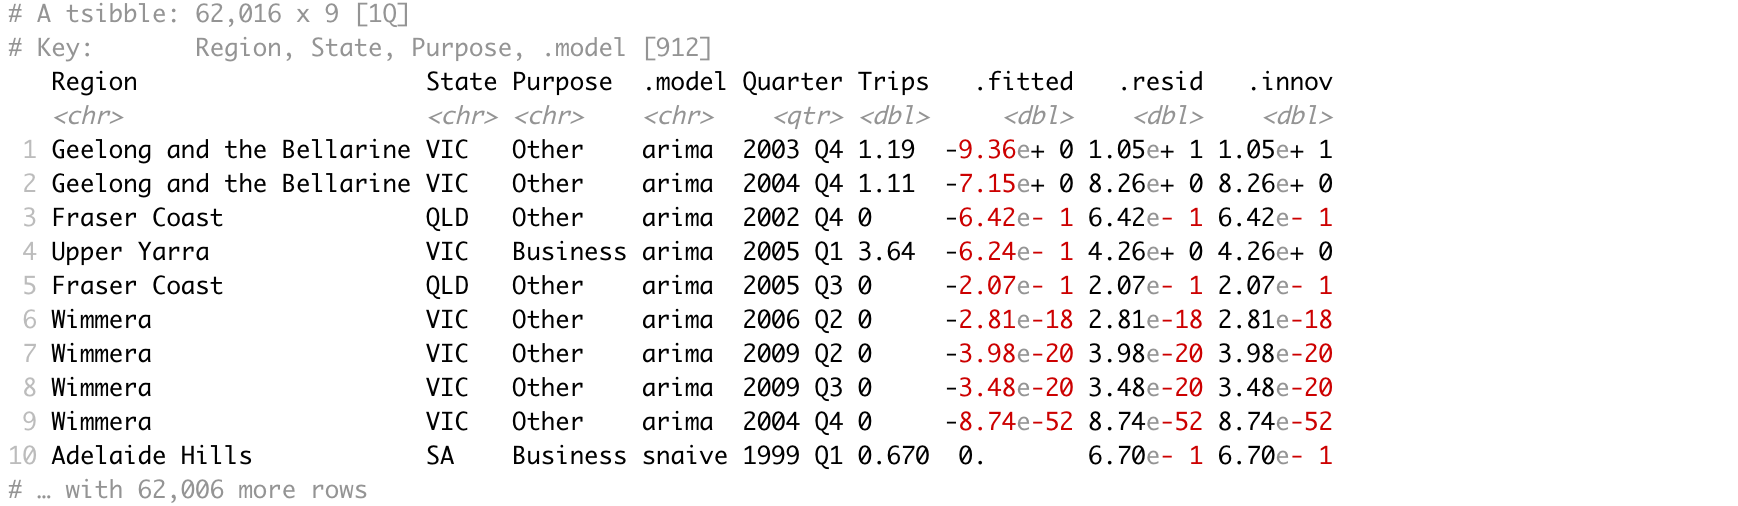
\includegraphics[width=110mm]{imgs/12_augment.png}
\end{figure}

\newpage

De la misma forma, se puede realizar un análisis análogo para los otros modelos. Por ejemplo para ETS se puede proporcionar la especificación del modelo, sus parámetros de smoothing y el AIC y BIC correspondiente a cada modelo entrenado:

\begin{lstlisting}
fit %>%
  filter(Region == "Snowy Mountains", Purpose == "Holiday") %>%
  select(ets) %>%
  report()
\end{lstlisting}

\begin{figure}[!h]
        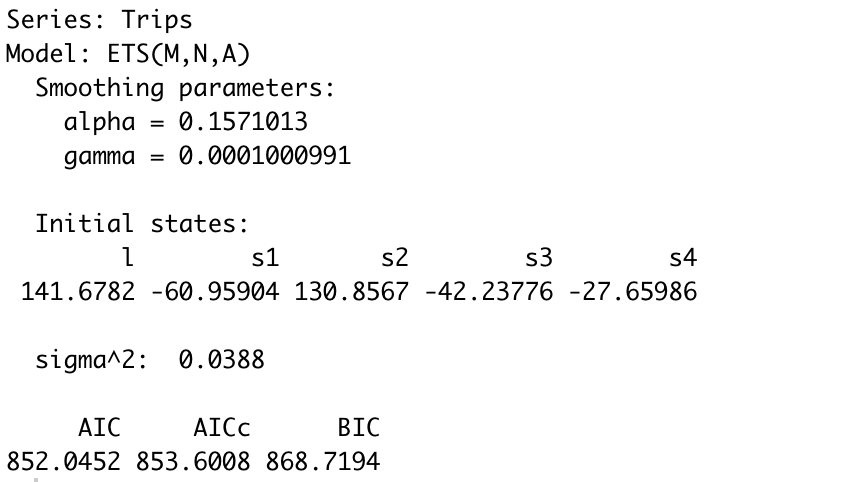
\includegraphics[width=75mm]{imgs/06_fit_ets.png}
\end{figure}

Por último para el Snaive también es posible exportar la especificación del modelo: 

\begin{lstlisting}
fit %>%
  filter(Region == "Snowy Mountains", Purpose == "Holiday") %>%
  select(snaive) %>%
  report()
\end{lstlisting}

\begin{figure}[!h]
        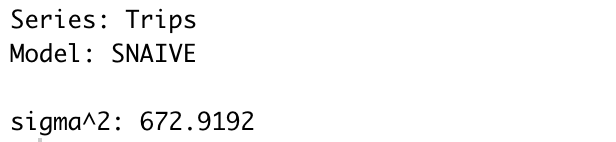
\includegraphics[width=55mm]{imgs/07_fit_snaive.png}
\end{figure}

Como se observa, gran parte de la paquetería está basada en \textit{fable}, por lo que es relevante compararlo con uno de los paquetes más usados en R: \textit{forecast}

\begin{itemize}
    \item \textit{fable} ocupa la estructura de tsibble y \textit{forecast} la estructura ts
    \item \textit{fable} puede manejar múltiples series de tiempo a la vez, mientras que \textit{forecast} solo una. 
    \item \textit{fable} permite entrenar varios modelos a la vez, mientras que \textit{forecast} solo uno 
    \item con \textit{fable} se puede manejar ensemble forecast facilmente, mientras con \textit{forecast} no es posible hacerlo
\end{itemize}

Ambos paquetes comparten un mismo autor (R. Hyndman), por lo que según otro de los autores del tidyverts, Mitchell O'Hara-Wild: ''\textit{fable} es considerada la siguiente iteración del paquete \textit{forecast}, el cual provee las herramientas y extensión necesitada para los retos actuales y futuros de las series de tiempo.''